%	 
\documentclass[a4paper,11pt]{book}

\usepackage{amsmath,amssymb,amsfonts,amsthm}    % Typical maths resource packages
\newcommand{\e}[1]{{\mathbb E}\left[ #1 \right]}

\DeclareRobustCommand{\bbone}{\text{\usefont{U}{bbold}{m}{n}1}}

\DeclareMathOperator{\EX}{\mathbb{E}}% expected value

\usepackage{graphicx}                           % Packages to allow inclusion of graphics
\usepackage{hyperref}                           % For creating hyperlinks in cross references
\usepackage{caption}
\usepackage{subcaption}
\usepackage{hyperref}
\usepackage{cite}

\usepackage[ruled,longend]{algorithm2e}

\usepackage[labelfont=bf]{caption}

\usepackage[]{algorithm2e}
\newlength\mylen
\newcommand\myinput[1]{%
  \settowidth\mylen{\KwIn{}}%
  \setlength\hangindent{\mylen}%
  \hspace*{\mylen}#1\\}
  
\usepackage[toc]{appendix}

%%%%%%%%%%%%%%%%%%%%%%%%%%%%%%%%%%%%% PYTHON CODE

% Default fixed font does not support bold face
\DeclareFixedFont{\ttb}{T1}{txtt}{bx}{n}{12} % for bold
\DeclareFixedFont{\ttm}{T1}{txtt}{m}{n}{12}  % for normal

\usepackage{listings}

%%%%%%%%%%%%%%%%%%%%%%%%%%%%%%%%%%%%% PYTHON CODE

\usepackage{verbatim}
\usepackage{titlesec}
\usepackage{floatrow}
\usepackage{float}
% -------------------------------
% --- some layout definitions ---
% -------------------------------
% define topline 	
\usepackage[automark]{scrpage2}
\pagestyle{scrheadings}
\automark{section}
\clearscrheadings
\ohead{\headmark}

% define citation style
\bibliographystyle{plain}

% define page size, margin size
\setlength{\headheight}{1.1\baselineskip}
\voffset=-2cm
\hoffset=-3cm
\textheight24cm
\textwidth15.5cm
\topmargin1cm
\oddsidemargin3cm
\evensidemargin3cm

% define line line spacing = 1.5
\renewcommand{\baselinestretch}{1.5}

\titleformat{\chapter}
  {\normalfont\LARGE\bfseries}
  {\thechapter}
  {.5em}
  {\MakeUppercase}
  [\vspace{.5ex}\titlerule]

\titlespacing*{\chapter}
  {0pt}
  {0pt}
  {20pt}

% define second level for `itemizing'
\renewcommand{\labelitemii}{-}

\begin{document}

% -------------------------------
% --- frontmatter: Title page ---
% -------------------------------

\thispagestyle{empty}
\begin{center}

{\LARGE{\bf Discriminative Machine Learning for Maximal Representative Subsampling}} \vspace{1.0cm}

%    {\Large{\bf One-Class Classification for Maximal Representative Sampling under Covariate-Shift}} \vspace{0.5cm}


    {\normalsize Bachelor's Thesis submitted\\\vspace{0.5cm}
    to}\\\vspace{0.5cm}
    {\normalsize{\bf Prof. Dr. Stefan Kramer}} \\
    and \\
    {\normalsize{\bf Prof. Dr. Andreas Hildebrandt}} \\\vspace{1cm}
\begin{figure}[ht]
	\begin{center}
		
\includegraphics[scale=0.20,angle=0]{fig/jgu}
	\end{center}
\end{figure}

    {\normalsize Johannes-Gutenberg University of Mainz \\
    Institute for Computer Science \\
    Chair of Data Mining\vspace{0.5cm}} 



    {\normalsize by \\
    {\bf Laksan Nathan} \\
    (2715043)} \vspace{1cm}


    {\normalsize in partial fulfillment of the requirements \\
    for the degree of \\
    {\bf Bachelor of Science} \\
    Mainz, January 17, 2019}

\end{center}



% -----------------------------
% --- frontmatter: Abstract ---
% ----------%-------------------
\newpage
\thispagestyle{empty}
%\section*{Abstract}
\chapter*{Abstract}
\thispagestyle{empty}
To allow statistical inference in social sciences, survey participants must be selected at random from the target population. When samples are drawn from parts of the population that are close to hand, subgroups might be over-represented. This leads to statistical analyses under sampling bias, which in turn may produce similarly biased outcomes. The present thesis uses machine learning to reduce this selection bias in a psychological survey using auxiliary information from comparable studies that are known to be representative. Discriminative algorithms are trained to directly characterize the divergence between representative and non-representative samples. The concept of positive-unlabeled learning is then applied to further improve results.


%Machine Learning models are trained to directly charaterize the divergence between representative and non-representative samples using auxiliary information from comparable studies that are known to be representative.



% -----------------------------
% --- frontmatter: Contents ---
% -----------------------------
\newpage
\tableofcontents
\addtocontents{toc}{\protect\thispagestyle{empty}}
\pagenumbering{gobble}
\clearpage

\titleformat*{\section}{\LARGE\bfseries}
\titleformat*{\subsection}{\Large\bfseries}

\newpage
\pagestyle{headings}
\pagenumbering{arabic}

\chapter{Introduction}

Psychological resilience is generally regarded as positive adaptation to past and ongoing exposure to potential negative effects of stressors. Accordingly, adaptation to stressful or adverse situation is a dynamic process with predictors that can differ between population groups. Within the discipline of developmental psychology, Tuescher and colleagues have provided prospective studies investigating the concept of resilience and its complex underlying mechanisms. As part of a doctoral dissertation, their studies aimed to validate the following research questions:

\begin{itemize}
    \item Does resilience have a positive effect on the willingness to participate in politics, specifically in election?
    \item Does the confrontation with positive or negative statements on politics for people with lower resilience have stronger effects on the willingness to participate in politics?
\end{itemize}

The research group did its poll by selecting people from Mainz, while trying to generalize to the entire German population. The survey data (GBS, n=587) tends to over-represent groups of higher income and higher education, since participants are primarily selected from an academic environment.

Therefore, the validity of assertions about the population beyond the original observation range is affected, even if statements are made conditional upon the available data. The basic premise for standard statistical conclusions, that the training and test set are drawn independently and identically (i.i.d.) from the same probability distribution, does not hold any more. Data sets are rarely generated under ideal conditions with bias pervasive in almost all empirical studies.

To get a complete picture of the subject, the research group consulted the department Data Archives for the Social Sciences. Their data archive service (GESIS) holds representative data of comparable studies in politics and psychology. The acquired sample (GESIS, n=4000) encompasses the German speaking population with permanent residence in Germany. 

This thesis is a practical application to reduce the sampling bias by selecting a maximal representative subsample (MRS) of GBS survey respondents with reference probability distributions from GESIS. The effects of positive and negative treatments on political participation are then analysed in the resulting MRS and compared to the initial GBS data [Fig. 1.1].

To evaluate the research questions to a certain required level of significance, it is inevitable to keep the exclusion of instances at a minimum. Pruning the GBS data in any way, narrows the data variance and thus the reach of subsequent studies. This is especially harmful since the initial GBS survey data is already small.

\begin{figure}[ht]
	\begin{center}
		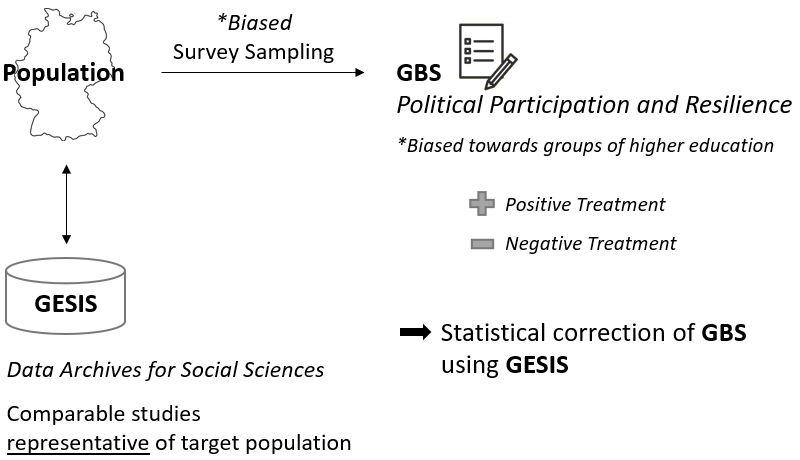
\includegraphics[scale=0.64,angle=0]{fig/overview}
		\label{project}
		\caption{Auxiliary information GESIS linked to GBS so that expected bias can be detected and corrected for. In addition, GBS contains an attribute for positive or negative treatment of survey participants for further analysis.}
	\end{center}
\end{figure}

Depending on the definition of MRS, there are two possible ways to tackle this problem:

\begin{enumerate}

\item Search algorithm with objective scoring function.

\item Try to avoid giving the synthesized data properties that makes it possible for a learning algorithm to distinguish synthesized from non-synthesized example such as if all the synthesized data comes from one of 20 car designs, or all the synthesized audio comes from only 1 hour of car noise. This advice can be hard to follow. 

\end{enumerate}

\section{Machine Learning for Complex Survey Data}

9.   Incorporate complex survey data features 

%http://ccsg.isr.umich.edu/index.php/chapters/statistical-analysis-chapter#nine

Several approaches exist to deal with positive and unlabeled data. The most straightforward one is to assume that all the unlabeled data are negative and simply apply standard machine learning techniques (Neelakantan, Roth, and McCallum 2015). A second approach is to select some of the unlabeled examples that are very different from the positively labeled ones and label them as negative. A classifier is then learned using the given positive examples and inferred negative examples (Liu et al. 2002; Li and Liu 2003; Yu, Han, and Chang 2004; Yu 2005; Li et al. 2009; Nguyen, Li, and Ng 2011). A third approach is to employ an evaluation metric that only uses positive, or positive and unlabeled data (Muggleton 1996; Lee and Liu 2003; Claesen et al. 2015a). Using this metric, one can tune for the best class weights or regularization settings (Lee and Liu 2003; Liu et al. 2005; Mordelet and Vert 2014; Claesen et al. 2015c). A final approach is to explicitly consider the class prior. It can be used to either adapt algorithms to incorporate this information during learning (Denis 1998; Liu et al. 2003; Zhang and Lee 2005; Denis, Gilleron, and Letouzey 2005; Elkan and Noto 2008) or as a preprocessing step to assign weights to the unlabeled examples (Elkan and Noto 2008). Because the class prior is often not known, several methods were proposed in the last decade to estimate it from the positive and unlabeled data (Elkan and Noto 2008; du Plessis and Sugiyama 2014; du Plessis, Niu, and Sugiyama 2015; Jain, White, and Radivojac 2016; Jain et al. 2016; Ramaswamy, Scott, and Tewari 2016) 

Both theoretical and practical results show that the out-of sample error increases proportionally to the distribution shift [2, 20]. To compensate for the degradation in performance, many techniques have been designed to reduce the effects of covariate shift.
% [1,4,9,10,12,15,16,17,18,19,21].	

\section{Outline}

I will frequently refer to decision tree theory. You will need a basic understanding of what they are to follow this text. Decision trees have performaned slightly outperformed comparable discriminative.

The remainder of this thesis is organized as follows. Section 2 starts with an initial data analysis step and focuses more narrowly on checking assumptions required for model fitting and hypothesis testing, i.e. handling missing values and making transformations of variables. Section 3 discusses the feasibility of learning in a binary classification setting. To estimate model performance in the absence of labeled negatives, standard evaluation metrics are adapted using an initial ranking model. Discriminative ensemble models are trained on positive and unlabaled data in Section 4 to label instances as representative that cannot be distinguished from the out-of-sample distribution. The resulting maximal representative subset of GBS is presented in Section 5 and compared to GBS and GESIS regarding political participation and resilience. Related work is discussed in Section 6 and Section 7 concludes.

\newpage
\chapter{Initial Data Analysis}\label{Sec:Initial Data Analysis}

In order to diagnose to what extent an algorithm suffers from sampling bias, it will be useful to have another dataset. Initial data analysis is conducted independently of the problem statements to understand what properties of the data differ between GBS and GESIS for matching attributes. A brief characterization of the data currently employed in the studies is given in this chapter. The GitHub repository further specifies the list of transformations that are sequentially applied to each group of features in order to prepare the inputs for survey comparisons. Preprocessing steps and methods used to evaluate outcomes are documented as well. Scaling methods that apply to both data sets, e.g: centering and scaling of skewed continuous features for SVMs, are not mentioned but can be deduced from code easily. If an attribute is removed at some point, it will only be mentioned in the relevant section.

\begin{figure}[ht]
	\begin{center}
		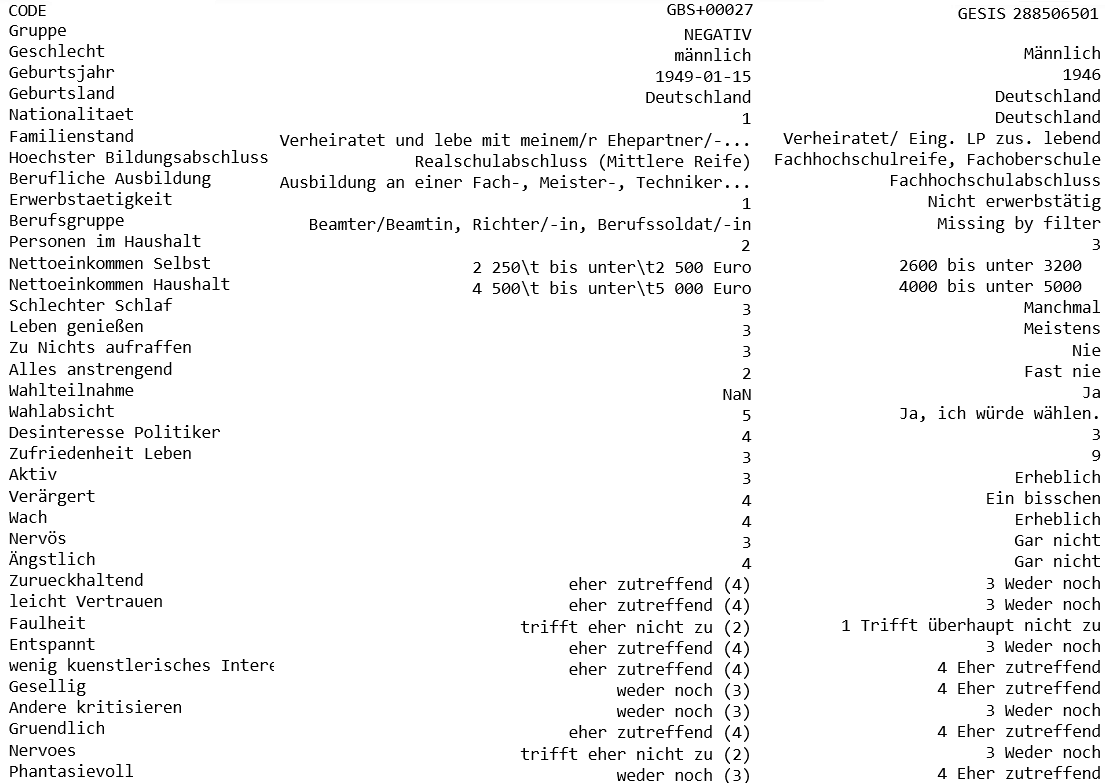
\includegraphics[scale=0.52,angle=0]{fig/values_compare}
		\label{std}
		\caption{GBS - GESIS attribute and value comparison. Not all attributes are used in every learning task. See GitHub documentation for more information.}
	\end{center}
\end{figure}

\section{Feature Selection and Data Imputation}

If not stated differently, deletion of rows is applied to every instance with missing values in GESIS to reduce the class imbalance in the later described classification problem. Missing values are sparse in GBS and can be imputed, e.g: with median substitution, with negligible effects. Mean substitution can not be used as this might lead to previously unseen values. Discriminative algorithms will then use these new values to distinguish GBS and GESIS that have been created by ill-considered data imputation. Note that the following figures represent the data after attribute and value matching described in Sec. 2.2. 

Fig. A.2 lends itself to first thoughts about whether missing data elements depend on observable attributes or occur entirely at random and is also able to detect functional dependencies in GESIS. Fig. A.3 summarizes the main observations from GBS. The correlation matrix with ratio -1 to +1 in Fig. A.4 is used as another way to visualize differences in GESIS and GBS and to further simplify preprocessing decisions. Potential bugs and issues can also be detected with this graph. 

\begin{figure}[h]
	\begin{center}
		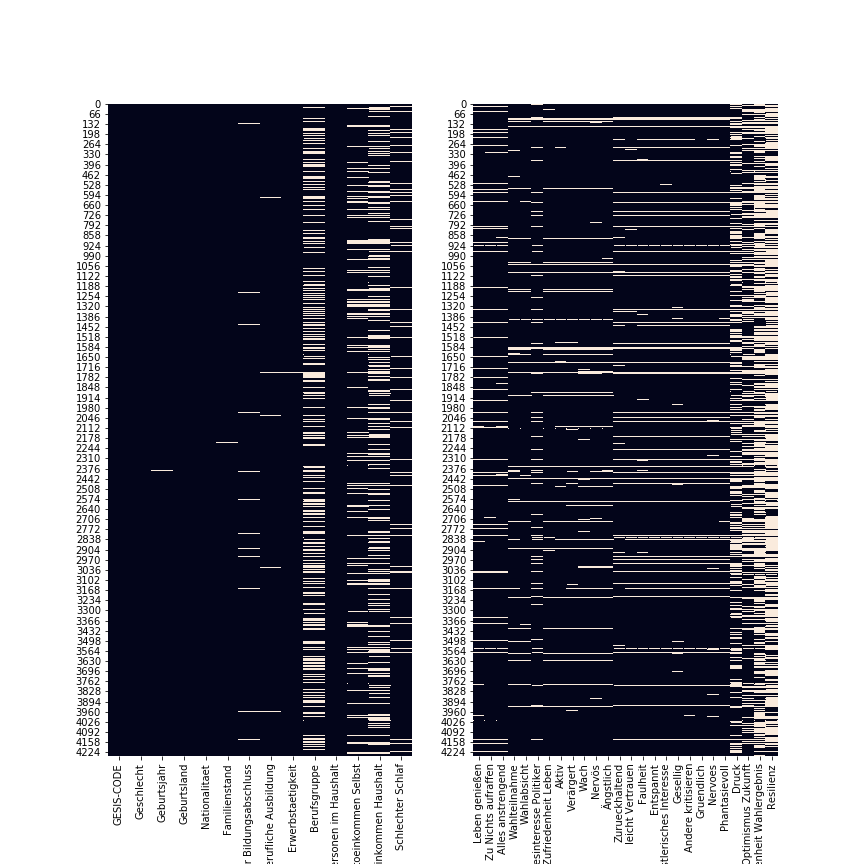
\includegraphics[scale=0.50,angle=0]{fig/gesis_missing}
		\label{gesis_miss}
		\caption{Missing values in GESIS. The attribute values of a participant are always known for "Geschlecht", "Geburtsland", "Geburtsjahr", "Nationalitaet", "Familienstand", "Personen im Haushalt". In contrast, the last three columns "Druck", "Optimismus Zukunft", "Zufriedenheit Wahlergebnisse" and "Resilienz" are almost always missing and are therefore removed from the analysis. Participants with missing BFI-10 elements are removed. Sample size will only be reduced slightly as missing values often occur for the same instance. These dependencies form a line pattern in the graph. "Berufsgruppe" was surveyed as a text field so that the column clearly suffers from ambiguous value mismatch. To include "Berufsgruppe" mappings need to be redefined first. For now, "Berufsgruppe" is removed. }
	\end{center}
\end{figure}

\begin{figure}[ht]
	\begin{center}
		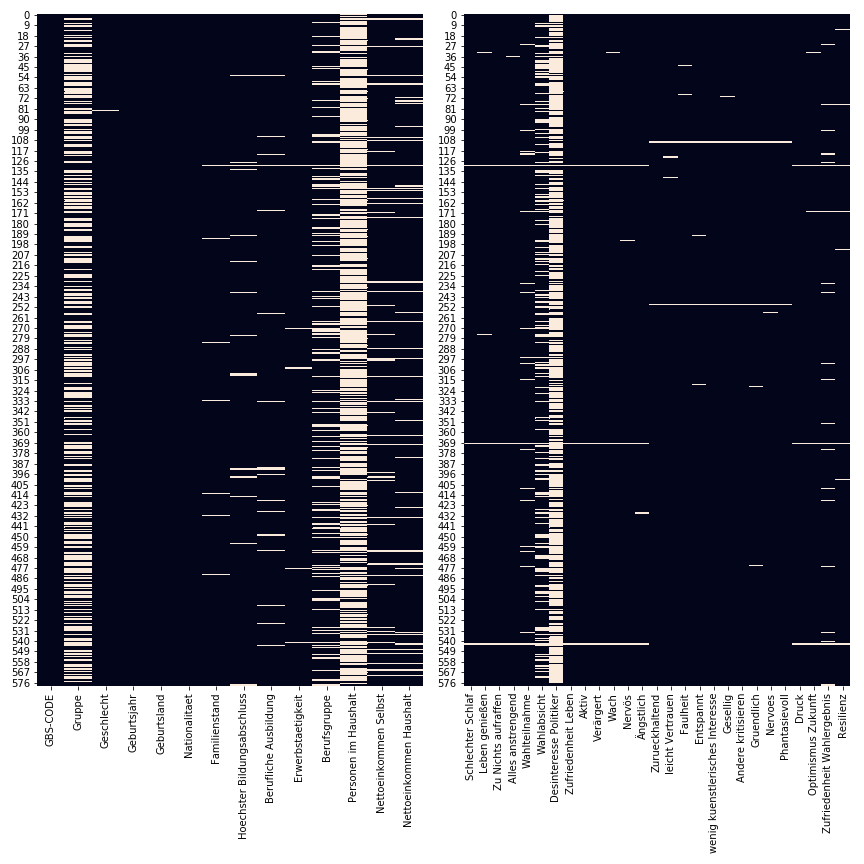
\includegraphics[scale=0.50,angle=0]{fig/gbs_missing}
		\label{gbs_miss}
		\caption{Missing values in GBS. There is one more attribute in "Gruppe". Not every participant received a positive a negative psychological treatment. Therefore, "Gruppe" is more likely to be missing than not. However, the absence of a value indicates no treatment rather than a missing positive or negative. "Gruppe" is not properly represented yet. "Desinteresse Politiker" is given by multiple data sources from different excel files. Some of them being the inverse of the attribute itself. The surey design regarding this issue is unclear to me. To incorporate "Desinteresse Politiker" the attribute(s) need to be imported correctly, if possible. Another import issue is given by "Personen im Haushalt". If the actual value is greater than one, the cell will be empty. To correct this, the corresponding csv-file needs to be fixed. The text field "Berufsgruppe" suffers on both ends, GBS and GESIS, due to current oversimplification of value and potential data mismatch.}
	\end{center}
\end{figure}

\begin{figure}[ht]
	\begin{center}
		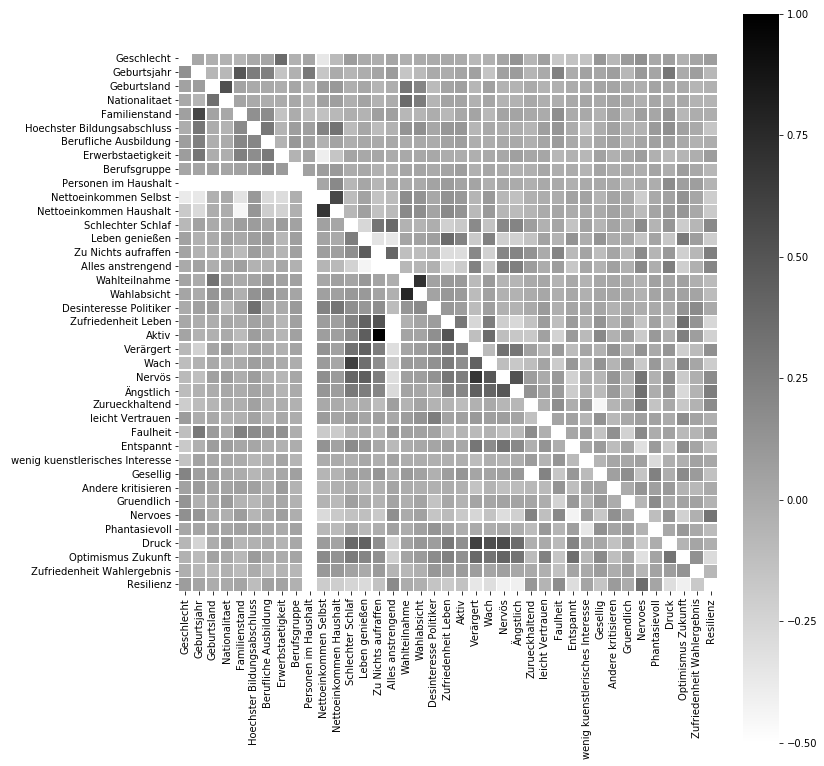
\includegraphics[scale=0.73,angle=0]{fig/correl}
		\label{corr}
		\caption{The upper right triangular matrix shows GESIS correlations while GBS correlations are shown in the lower left. The main diagonal should not be confused with white squares. These trivial combinations are simply excluded and not colored black. As can be seen "Personen im Haushalt" in GBS can not be calculated, since there is only one possible value. "Nettoeinkommen Selbst" and "Nettoeinkommen Haushalt" are highly correlated but not removed or handled at all. I will keep this in mind, when facing the naive bayes assumption in the learning process. Entropy-based mutual information in "Wahlteilnahme" and "Wahlabsicht" have led to almost perfect classification performances in predicting political participation. "Wahlabsicht" is therefore removed.}
	\end{center}
\end{figure}

\section{Perspectives on Response Styles}

In survey analysis, scales measuring attributes need to be reliable and valid. Therefore, GBS and GESIS almost entirely use already tested scales from the literature.

\subsection{Likert-Type Scale}

The Big Five is an empirically-derived model of human personality and psyche. When factor analysis is applied to personality survey data, five clusters of traits consistently emerge. The BFI-10 is a 10-item scale measuring the Big Five personality traits, two BFI items for each dimension, representing both the high and low pole of each factor [Fig X]. Likert scales are the most frequently used instruments in GBS and GESIS. They consist of statements which measure the intensity of one's estimation towards the preceding statement. Respondents are asked to rate the BFI-10 items on a level of agreement on a consistent rating scale ranging from "Strongly Agree (5)" to Strongly Disagree (1)" for all items in both survey.

\begin{figure}[H]
	\begin{center}
		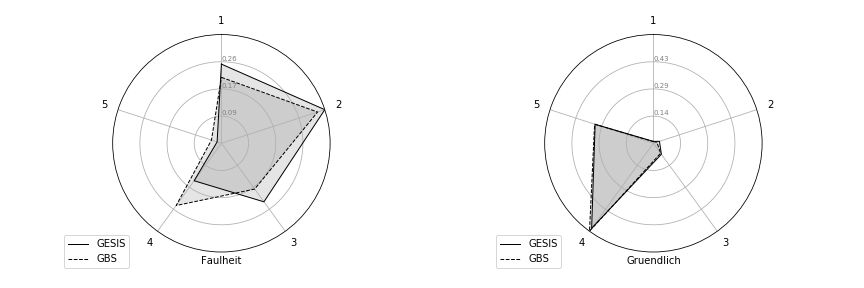
\includegraphics[scale=0.52,angle=0]{fig/Conscientiousness_figure}
		\label{Conscientiousness}
		\caption{Conscientiousness is the degree of organization, self-regulation, and responsibility one exhibits. \textit{"I see myself as someone who tends to be lazy."}(left). \textit{"I see myself as someone who does a thorough job."}(right). The graphs are almost identical for the Likert item "Gruendlich". Respondents specify their level of disagreement for "Faulheit" more in GBS.}
	\end{center}
\end{figure}

\begin{figure}[ht]
	\begin{center}
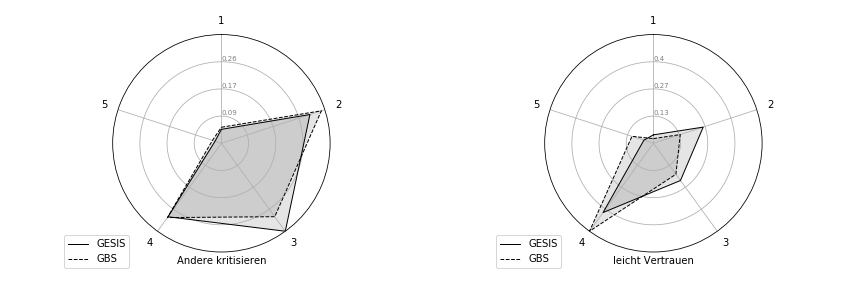
\includegraphics[scale=0.42,angle=0]{fig/Agreeablenessfigure} \\
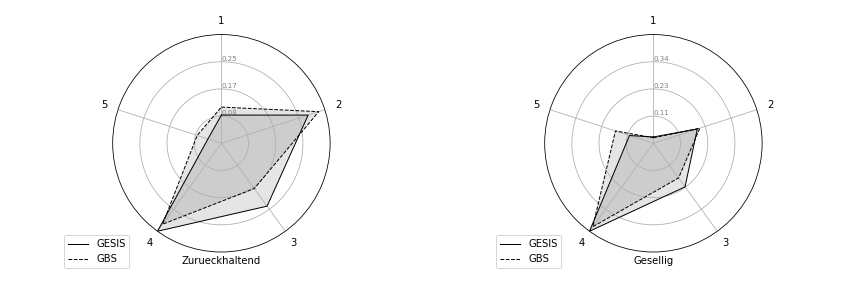
\includegraphics[scale=0.31,angle=0]{fig/Extraversionfigure} \\
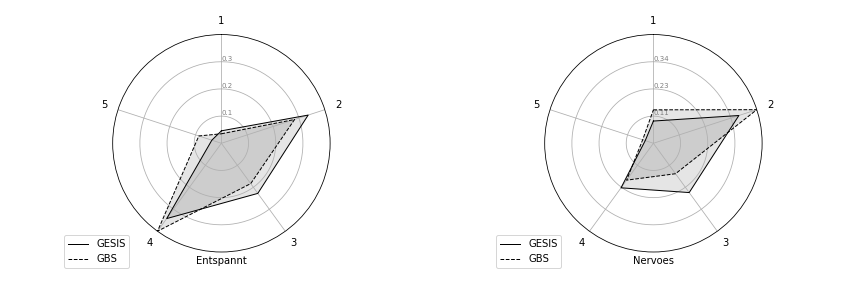
\includegraphics[scale=0.31,angle=0]{fig/Neuroticismfigure} \\
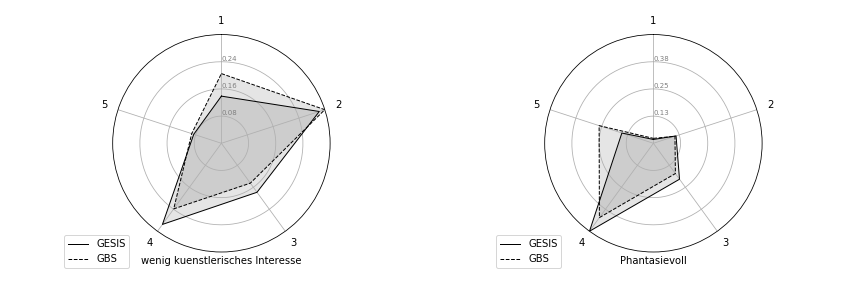
\includegraphics[scale=0.31,angle=0]{fig/Opennessfigure} \\
\vspace{0.75cm}
\caption{Agreeableness is the measure of one's cooperation, empathy, and willingness to trust and help others. Openness estimates whether one is hesitant or eager about new objects or situations. Extraversion refers to level of sociability, seeking and enjoyment of social contact, and energy and assertiveness in social situations. Neuroticism is characterized by easily experiencing negative emotions, and a poor coping response to those emotions. The cyclic structure of the chart, i.e. "Strongly Disagree" next to Strongly Agree", provides a vivid example for the central-tendency bias across all items.}
\end{center}
\end{figure}

is still ongoing debate on whether to use a Likert scale item as categorical or numeric feature. The intervals between positions on the scale are monotonic but never so well-defined as to be numerically uniform increments. A "Strongly Agree (5)" response indicates more agreement than "Agree", but it does not show agreement that is five times stronger than "Strongly Disagree (1)". 

There is an underlying measurement continuum, but  
This project treats the responses as if they fell on an interval scale.

Figure X. shows the response distribution of values for "Conscientiousness" of GBS and GESIS participants (see Appendix for a visualization of distribution shifts in "Agreeableness", "Openness", "Extraversion" and "Neuroticism").

Since GESIS and GBS analyse on a group level should be relatively insensitive to problems that may arise.

In all these cases each aggregate measure (perhaps the mean) is based on many individual responses (e.g., n=50, 100, 1000, etc.). In these cases the original Likert item begins to take on properties that resemble an interval scale at the aggregate level.
life satisfaction of states or countries,
job satisfaction of departments,

\subsection{Data Mismatch}

John Tukey wrote otherwise (back in 1960) in a monograph "Data Analysis and Behavioral Science" (published in Collected Works v. III). One result he obtained is that if you're getting better than about 10percent test-retest agreement, your scale isn't narrow enough!

[1] It is confirmed that different numbers of rating bars in a subjective rating scale can have significant effects on the subjective measurement, thus the assessment of the Big Five dimensions of personality.

\begin{table}[ht]
    \begin{center}
            {\footnotesize
            \begin{tabular}{l|c|ccccccccc}
                \hline \hline
		Raw Data & GESIS & 1 & 2 & 3 & 4 & 5 & 6 \\
                     & GBS & 1 & 2 & 3 & 4 & 5 & \\
                \hline
		Max Scaler & GESIS & 0.83 & 1.7 & 2.5 & 3.3 & 4.2 & 5.0 \\
                     & GBS & 1 & 2 & 3 & 4 & 5 & \\
                \hline
		Min-Max Scaler & GESIS & 1 & 1.8 & 2.6 & 3.4 & 4.2 & 5 \\
                     & GBS & 1.0 & 2.25 & 3.5 & 4.75 & 6.0 & \\
                \hline
		Cut-Off Mapping & GESIS & 1 & 2 & 3 & 4 & 5 & 5 \\
                     & GBS & 1 & 2 & 3 & 4 & 5 & \\
\hline \hline
            \end{tabular}}
        \caption{Different value scalings of attribute "Desinteresse Politiker".}
\label{Tab:DescripStatsRawData}
\end{center}
\end{table}

Shortcomings in attribute mappings may result in inappropriate representation and incorrect conclusions.

\begin{table}[ht]
    \begin{center}
            {\footnotesize
            \begin{tabular}{l|c|ccccccccc}
                \hline \hline
		attribute & GBS values & GBS values count &  GBS values & GBS values count \\
                \hline \hline
                     Wach & 4 & 311 & Einigermassen & 1697 \\
                     & 3 & 183 & Erheblich & 1389 \\
                     & 2 & 66 & Ein bisschen & 467 \\ 
              	& 1 & 14 & Aeusserst & 367 \\	
		& -1 & 1 & Gar nicht & 184 \\		
		& -9 & 1 & & \\
	     \hline \hline
            \end{tabular}}
        \caption{Caption.}
\end{center}
\end{table}

\begin{figure}[ht]
	\begin{center}
		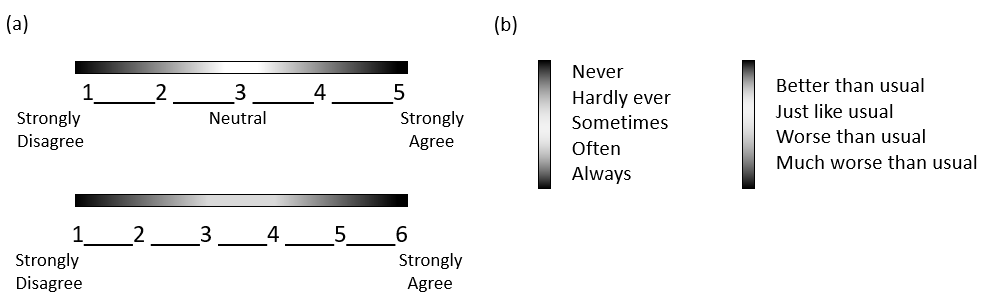
\includegraphics[scale=0.50,angle=0]{fig/scales}
		\label{6_5}
		\caption{Example of a Likert item discrepancy. GBS uses an odd number of responses with a "neutral" option, such as "no opinion", "neither agree nor disagree" or some phrase to that effect. In contrast, there is an even number of responses for this item in GESIS encouraging participants to voice a positive or negative opinion.}
	\end{center}
\end{figure}

\begin{figure}[ht]
	\begin{center}
		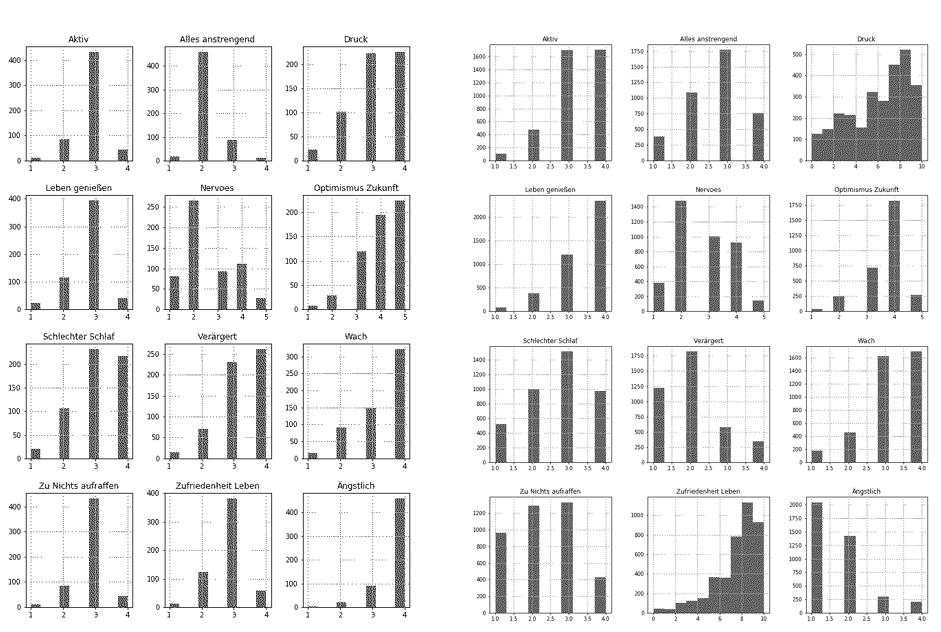
\includegraphics[scale=0.62,angle=0]{fig/histo}
		\label{std}
		\caption{GESIS hists.}
	\end{center}
\end{figure}

Figure X shows an example of such as a statement.

In some cases, an additional "opt-out" option is provided for those respondents who truly cannot respond in GBS only.


\newpage
\chapter{Feasibility of Learning}\label{Sec:Feasibility of Learning}

No practical amount of data can distinguish between two distributions, thus instances of GBS can not be proven to come from GESIS. However, machine learning allows to infer the conditional probability of \textit{'GBS participant is representative'} given the survey data within a probabilistic framework. A well-defined learning problem involves a number of design choices, including selecting the target function to be learned, a representation for this target function, and an algorithm to learn from the source of training experience \cite{tom}. This paper defines key terminology of the theoretical aspects of survey analysis and machine learning. The MRS algorithm is then formulated as positive-unlabeled learning problem in addition to traditional machine learning.

\section{Sampling Bias}

Variables considered in the GBS study must accurately reflect the populations characteristics. That is, every element of the population has a known non-zero chance of being selected. This includes people whether or not they choose to take part in the survey. Results can then be used to make estimates for not only the sample itself but also the target population. A sampling method is called biased if it systematically favors some people over others, e.g. by oversampling people with strong opinions and undersampling people who do not care much about the topic of the survey \cite{west}.

Sampling bias is often referred to as selection bias or sample selection bias. I will stick to the more descriptive term sampling bias. It underlines the fact that the bias arises in how the data was sampled. Also, the use of the term becomes less ambiguous, because there exists another notion of selection bias in the context of model selection. This type of bias is usually referred to as bad generalization, where the performance of the selected hypothesis is overly optimistic \cite{yaser}.

\section{The Problem of Overfitting}

Overfitting stands out as one of the biggest challenges for machine learning. It is not exclusive to machine learning but rather a fundamental problem across science and is at the very heart of the dangers of statistical inference. Hypothesis \(h\) in \(H\) overfits training data if there exists an alternative hypothesis \(\bar{h}\) in \(H\) such that \(errorTrain(h) < errorTrain(\bar{h})\) and \(errorD(h) > errorD(\bar{h})\), where \(errorTrain(h):=\) error of hypothesis \(h\) over training data and \(errorD(h):=\) error over entire distribution \(D\) of data. A hypothesis overfits the training examples if some other hypothesis that fits the training examples less well actually performs better over the entire distribution of instances \cite{yaser}.

When overfitting occurs, the learned hypothesis is very good at calculating the answers for the given data, but much less so for new instances it encounters. In a sense, the machine learning algorithm has become fixated on unimportant features of the training data overlooking the big picture. It often occurs when the algorithm has too many options to play with in designing its mappings, an approximation of the target function. The freedom to tune parameters and add complexity until it exactly matches the training data, rather than looking for large, systematic patterns leads to high variance \cite{yaser}.

The expected prediction error at any given data point \(x_0\), the generalization error, can be decomposed as follows \cite{ian}: 
\begin{align*}
Err(x_o) &= \EX[(Y - \bar{f}(x_0))^2 \mid X = x_0] \\
& =  \sigma^2_\epsilon + [\EX\bar{f}(x_0) - f(x_0)]^2 + \EX[\bar{f}(x_0) - \EX\bar{f}(x_0)]^2\\
& =  \sigma^2_\epsilon + Bias^2(\bar{f}(x_0)) + Var(\bar{f}(x_0)) \\
& = Irreducible Error + Bias^2 + Variance
\end{align*}

The bias and variance terms make up the error of \(\bar{f}(x_0)\) in estimating \(f(x_0)\). The bias component is the squared difference between the true mean \(f(x_0)\) and the expected value of the estimate \([\EX\bar{f}(x_0) - f(x_0)]^2\), where the expectation averages the randomness in the training data. The variance term refers to the amount by which the estimate of the target function would change if it was estimated using a different training data set. Ideally the estimate for the underlying pattern should not vary too much between training sets. More generally, as the model complexity is increased, the variance tends to increase and the squared bias tends to decrease. The opposite behavior occurs as the model complexity is decreased. The first term in this expression is the irreducible error, a combination of stochastic and deterministic noise. More precisely, stochastic noise are fluctuations or measurement errors that can not be modelled. Re-measuring \(y_n\) changes this component. Deterministic noise is the part of the target function that can not be represented. Changing \(H\) changes this component. With a single dataset \(D\) and fixed \(H\) it is impossible to distinguish \cite{yaser}.  

\section{Discriminative Learning} 

With the definitions above, a model is not necessarily overfitting because of poor generalization performance. It simply gets much more complicated to analyse sources of error in a covariate-shift setting. To evaluate the actual performance of a model, the given data samples must be split properly.

Several approaches exist to deal with positive and unlabeled data. The most straightforward one is to assume that all the unlabeled data are negative and simply apply standard machine learning techniques (Neelakantan, Roth, and McCallum 2015).

The error rate on the training data, the resubstitution error, as turned out to be overly optimistic, is not a good indicator of performance on future data. The holdout estimate can be made more reliable by repeating the process with different subsamples. The error rates on the different iterations are averaged to yield an overall error rate.

There is almost always not enough data available to partition it into separate training and test sets without losing significant modelling or testing capability. In these cases, a fair way to properly estimate model prediction performance is to use cross-validation as a powerful general technique \cite{ian}.

The intuition for these results comesfrom the fact that in many practical situations, the posteriordistributions in traditional and non-traditional setting pro-vide the same optimal ranking of data points on a given testsample (Jain et al. 2016; Jain, White, and Radivojac 2016).

\begin{figure}[ht]
	\begin{center}
		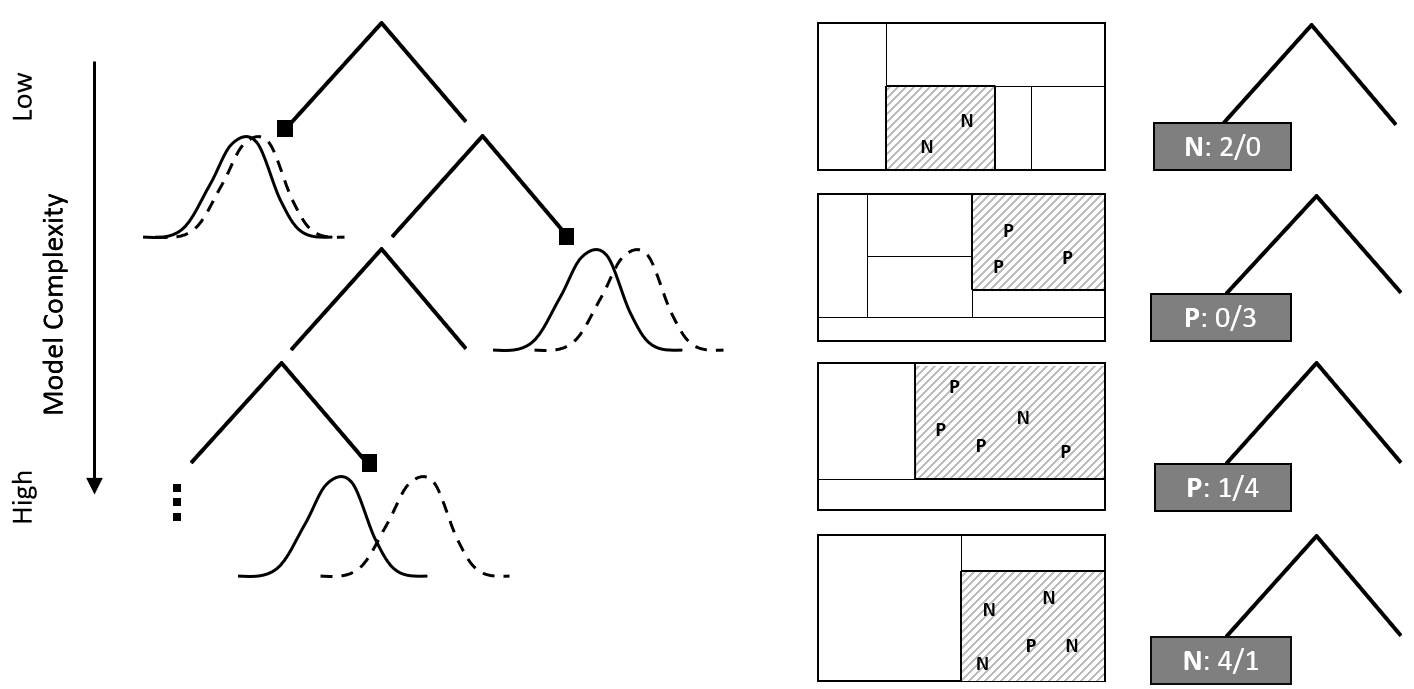
\includegraphics[scale=0.40,angle=0]{fig/tree3}
		\label{project}
		\caption{.}
	\end{center}
\end{figure}

\section{Learning from Positive and Unlabeled Data}

To further reduce the variance of the error estimate, each class is sampled with approximately equal proportions in both datasets, a technique called stratification. 

We have shown the effect of resampling contaminated sets and provided some basic insight into the mechanics of bagging. We will now link these two elements to justify bagging approaches in the context of contaminated training sets. Its usefulness can be considered by both the variance reduction argument of Bauer and Kohavi [4] and equalizing the influence of training points as described by Grandvalet [24]. Variance reduction. Resampling a contaminated set yields different levels of contamination in the resamples as explained in Section 3.1. Varying the contamination between base model training sets induces variability between base models without increasing bias. This observation enables us to create a diverse set of base models by resampling both P and U. The variance reduction of bagging is an excellent mechanism to exploit the variability of base models based on resampling [4, 10]. In the context of RESVM, a tradeoff takes place between increased variability (by training on smaller resamples, see Figure 1) and base models with increased stability (larger training sets for the SVM models).

PU learning is a semi-supervised technique that does not make the simplifying assumption of GBS instances being negative. Instead, a one-class classifier is trained on GESIS only. [...] This can result in even better assessment. [Read Literature] - Imporance weighted cross validation and pu learning with proper assessment. State-of-the-art techniques in positive-unlabeled learningtackle this problem by treating the unlabeled sample as neg-atives and training a classifier to distinguish between la-beled (positive) and unlabeled examples. Surprisingly,for a variety of performance criteria, non-traditional classi-fiers achieve similar performance under traditional evalua-tion as optimal traditional classifiers (Blanchard et al. 2010;Menon et al. 2015). 

\vspace{0.4cm}

\begin{algorithm}[H]
\caption{PU training procedure}\label{alg:alg}
\vspace{0.2cm}
\KwIn{\(P\): set of positive instances (GESIS)}
\myinput{\(U\): set of unlabeled instances (GBS)}
\myinput{\(n_{models}\): number of base models in ensemble}
\myinput{\(n_P\): size of bootstrap sample of \(P\)}
\myinput{\(n_U\): size of bootstrap sample of \(U\)}
\KwResult{Scoring function \(f:U \rightarrow \) $\mathbb{R}$}
Initialize: 
\(f(x) \leftarrow 0\) and 
\(c(x) \leftarrow 0\)\\
\For{t = 1 to \(n_{models}\)}{
\hfill \\
  Draw a bootstrap sample \(P_t\) of size \(n_P\). \\
  Draw a bootstrap sample \(U_t\) of size \(n_U\). \\
  Train classifier \(f_t\) to discriminate \(P_t\) against \(U_t\). \\
  For any \(x \in U \backslash U_t\), update: \\
\(f(x) \leftarrow f(x) + f_t(x),\) \\ 
\(c(x) \leftarrow c(x) + 1\) \\
\vspace{0.2cm}}
Return: \(s(x) = f(x)/c(x)\)
\vspace{0.3cm}
\end{algorithm}

\begin{comment}
\begin{algorithm}[H]
\caption{Transductive bagging PU learning}\label{alg:alg2}
\KwIn{\(P\): set of positive instances (GESIS)}
\myinput{\(U\): set of unlabeled instances (GBS)}
\myinput{\(K_P\): size of bootstrap samples, \(T\): number of base models in ensemble}
\KwResult{Ranking score \(s:U \rightarrow \) $\mathbb{R}$}

\For{t = 1 to \(T\)}{
 Draw a bootstrap sample \(P_t\) of size \(K_P\). \\
 Train classifier \(f_t\) to discriminate \(P_t\) against \(U\). \\
 For any \(x \in U \backslash U_t\), update:
\[f(x) \leftarrow f(x) + f_t(x),\]
\[n(x) \leftarrow n(x) + 1\]
}
Return \[s(x) = f(x)/n(x)\]

\end{algorithm} 
\end {comment}

The most extensively studied and widely used performance evaluation in binary classification involves estimating the Receiver Operating Characteristic (ROC) curve. The ROC curve plots the true positive rate (recall) of a classifier as a function of its false positive rate (Fawcett 2006) over a range of decision thresholds. Furthermore, AUC has a meaningful probabilistic interpretation that is used to  the ability of the classifier to separate classesand is often used to rank classifiers (Hanley and McNeil1982). the widely-accepted evaluation approaches us-ing ROC curves are insensitive to the variation ofraw prediction scores unless they affect the ranking.

Let \(f\) be the true distribution over the input space \(X\) from which unlabeled data is drawn. With distributions \(f_1\) and \(f_0\) of the positive and negative examples, respectively, it follows that
\[f(x) = \alpha f_1(x) + (1-\alpha)f_0(x)\]
with positive class prior \(\alpha \in [0,1], x \in X\).

Consider the binary classification problem from input \(x \in X\) to output \(y \in Y\) (representative: '\(1\)', not representative: '\(0\)'). The learning objective is to discriminate between \(X_p\) drawn according to \(f_1\) and \(X_u\) drawn according to \(f\)  and recover its performance estimate in the traditional setting, i.e. evaluating the decision boundary between positive and negative data.

Recall \(\gamma\), false positive rate \(\eta\) and precision \(\rho\) are defined as: \(\gamma = P[\hat{Y} = 1| Y = 1]\), \(\eta = P[\hat{Y} = 1| Y = 0]\) and \(\rho = P[Y = 1| \hat{Y} = 1]\), where \(\hat{Y}\) is an estimate of the true class label \(Y\). TPR \(\gamma\) can be estimated directly, because \(X_p\) was sampled from \(f_1\), while this does not hold true for \(\eta\) given the absence of samples from \(f_0\). 
\begin{gather*}
\gamma = \e{f_1[h(x)]} = \frac{1}{|X_p|} \sum\nolimits_{x \in X_p} h(x) \\
\hat{\eta}^{pu} = \e{f[h(x)]} = \frac{1}{|X|} \sum\nolimits_{x \in X} h(x)
\end{gather*}

The area under ROC curves \(AUROC^{pu}\) so far could only be estimated for the positive versus unlabeled classification by plotting \(\gamma\) and \(\hat{\eta}^{pu}\). To calculate \(AUC\) from \(AUC^{pu}\), S. Jain et al. (2015) express \(\eta\) in terms of \(\hat{\eta}^{pu}\) and \(alpha\) and provide a full derivation from the probabilistic definition of the AUC with

\[\eta = \frac{\hat{\eta}^{pu} - \alpha \gamma}{1 - \alpha}\] so that

\[AUC = \frac{AUC^{pu} - \frac{\alpha}{2}}{1 - \alpha}\] proving

\[AUC > AUC^{pu} \iff AUC^{pu} > \frac{1}{2}\].
\newpage
\chapter{Results}\label{Sec:Results}

\section{Maximal Representative Subsample}
 
There is almost always not enough data available to partition it into separate training and test sets without losing significant modelling or testing capability. In these cases, a fair way to properly estimate model prediction performance is to use cross-validation as a powerful general technique[5].

The overly optimistic resubstitution error, is not a good indicator of model performance. To evaluate the actual performance of a model, the given data samples need to be split. The proper procedure uses three sets: training data, validation data, and test data [2]. The holdout method is the most common approach to get a reliable performance estimation: A certain amount of data is reserved for testing while the remainder is used for the actual training. Because the method is very fast, it is useful to use when the algorithm is slow to train and the dataset is large. Training and test sets might not be representative of the same underlying distribution, e.g. class hardly represented in the test set.

The holdout estimate can be made more reliable by repeating the process with different subsamples. The error rates on the different iterations are averaged to yield an overall error rate. To further reduce the variance of the error estimate, each class is sampled with approximately equal proportions in both datasets, a technique called stratification. Figure X shows the results on the GFI-10 data.

\subsection{Fraction of Positives}

Estimating Positive Class Prior with One-Class SVMs. Using the One-Class SVM and its ability to capture the shape of the data set, hence performing better when the data is strongly non-Gaussian, i.e. with two well-separated clusters;

\begin{figure}[ht]
	\begin{center}
		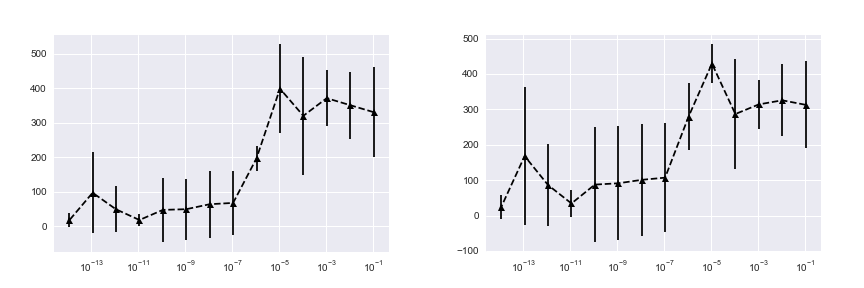
\includegraphics[scale=0.55,angle=0]{fig/occfigure}
		\label{occ}
		\vspace*{-1.0cm}
		\caption{Tuning parameter \(nu\) that controls the trade-off between the fraction of non-representative samples and the number of support vectors in one-class SVM. More than 0.73 of GBS (right) are classified as representative with high confidence (low sdt) for the optimal value \(nu = 10^{-5}\).}
	\end{center}
\end{figure}

\subsection{ROC and puROC Evaluation}

\begin{figure}
\centering
		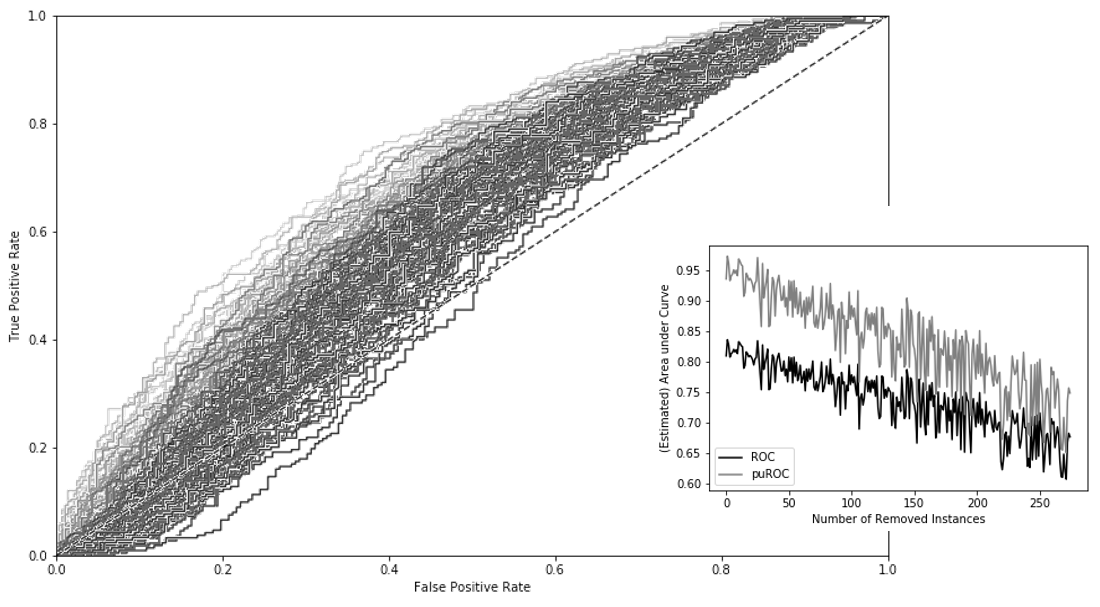
\includegraphics[scale=0.50,angle=0]{fig/res1}
   \label{fig:Ng1} 
\end{figure}

\section{Political Participation and Resilience}

In modelling a political participation process, a computer program is designed to approximate the likelihood of a person going to vote on election day. Ideally, for every instance with unknown political interest and willingness to participate, there is enough data of people of similiar demographics, socioeconomics and psychological traits to generalize from. 

\begin{figure}
\centering
\begin{subfigure}[b]{0.8\textwidth}
		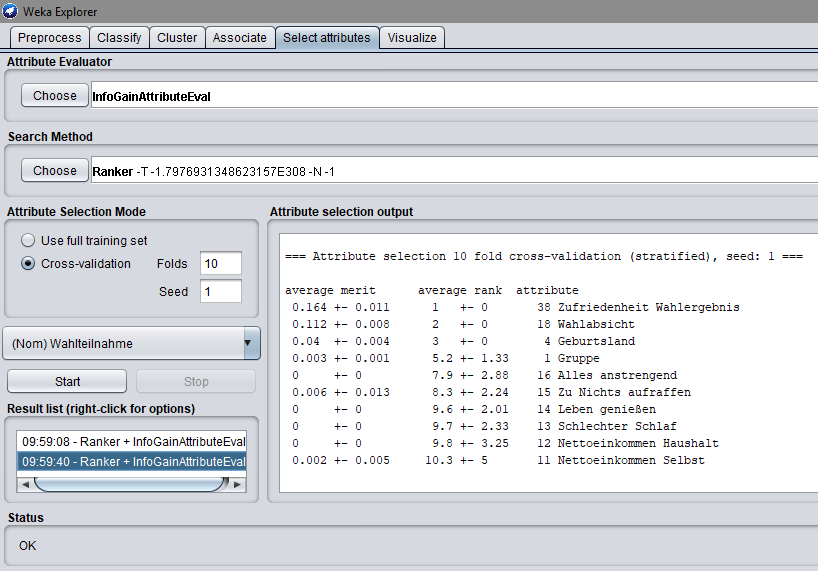
\includegraphics[scale=0.55,angle=0]{fig/weka_gbs}
   \label{fig:Ng1} 
\end{subfigure}

\begin{subfigure}[b]{0.8\textwidth}
\vspace{0.55cm}
		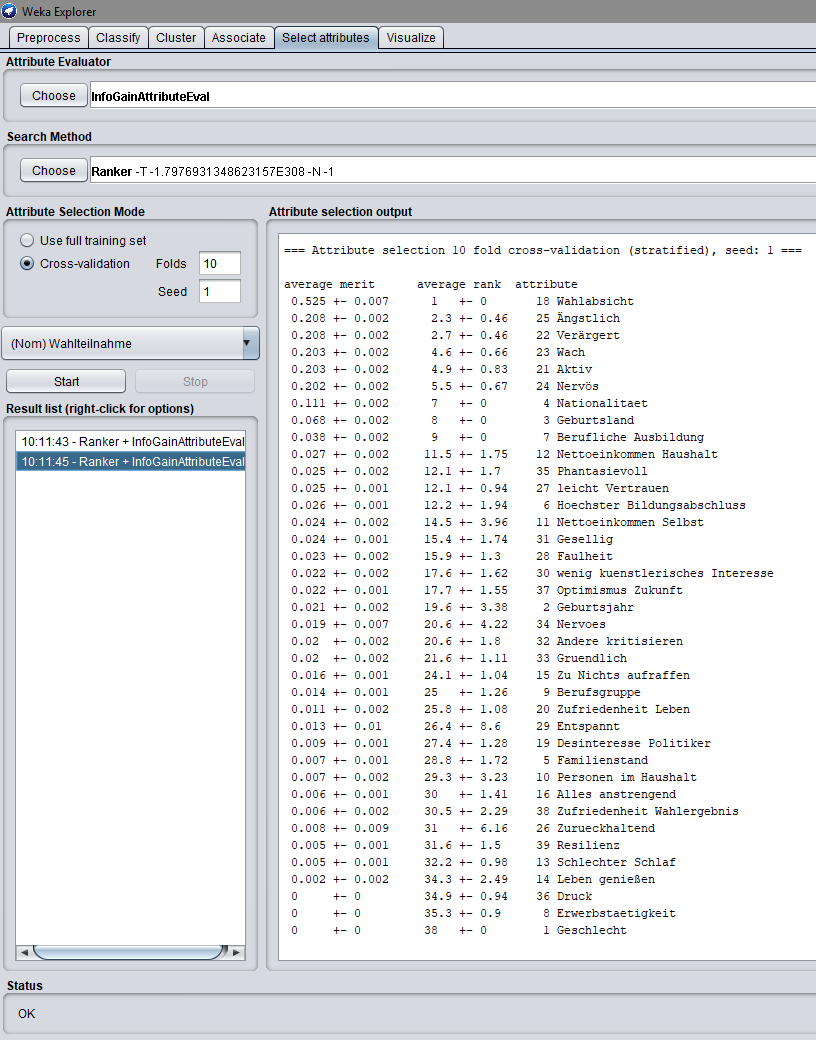
\includegraphics[scale=0.55,angle=0]{fig/weka_gesis}
   \label{fig:Ng2}
\end{subfigure}
\vspace{0.35cm}
\caption{Feature importance GBS (n=579) and GBS MRS (n=280) in classification of political participation "Wahlteilnahme".}
\end{figure}


\newpage
\chapter{Future Work}\label{Sec:Future Work}

Many different adaptations, statistics, and experiments have been left for the future due to lack of time, i.e. data matching and transformation with real data have been very time consuming. Controlled environments are needed to observe the behavior of the proposed algorithm.

For one thing, future work concerns deeper analysis of the proposed sampling method, in particular, experiments on synthezised data. The Synthetic Minority Over-sampling TEchnique (SMOTE [9]) is a very popular oversampling method that creates synthetic minority class instances. The SMOTE instances are linear combinations of two similar instances from the minority class (\(x\) and \(x^{R}\)) and are defined as: \(s = x + u (x^{R} - x) \) with \(0 \geq  u \geq 1\). \(x^{R}\) is randomly chosen among the \(k\) nearest neighbors of \(x\) belonging to the minority class. SMOTE can be used to validate the MRS procedure by simulating the problem at hand.

Specific regions in the feature space are first over-sampled using SMOTE, before they are under-sampled by MRS. Experiments with multiple such synthesized data, with oversampling ratio ranging from high to low, might support the proposed procedure with greater evidence. The initial data sets are then compared to the result sets. GESIS is particularly well suited to artificially recreate the initial problem as visualized in Figure 5.1. It is only necessary to try to avoid giving the synthesized data properties that makes it possible for a learning algorithm to distinguish synthesized from non-synthesized example. This mechanism would for instance aid to compare classification results more easily.

\begin{figure}[ht]
	\begin{center}
\vspace{0.5cm}
		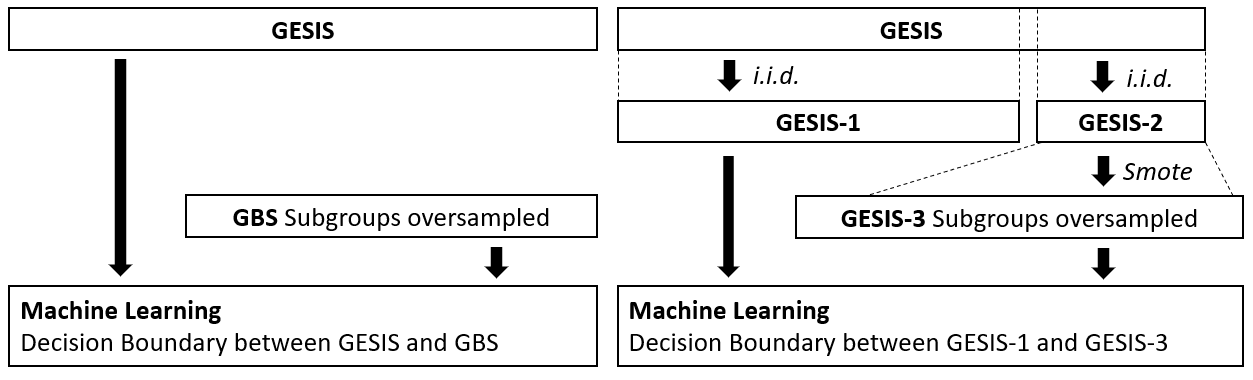
\includegraphics[scale=0.41,angle=0]{fig/procedure2}
		\label{std}
		\caption{Artificial data synthesis to overrepresent subgroups of GESIS. True negatives are removed from the MRS with positive classes GESIS (left) and GESIS-1 (right). Oversampled instances can easily be marked as such for result set comparisons.}
	\end{center}
\end{figure}

The main criteria considered in this work has been the area under the ROC curve. Having a single-number evaluation metric speeds decision-making when selecting among non-representative instances. It gives a clear preference ranking among all of them, and therefore a clear direction for progress. To enable a basis for a more informed exclusion of instances, another important performance criterion generally used in information retrieval could be added. The F-Measure, including summary statistics derived from the precision-recall curve, may be preferred to ROC curves when classes are heavily skewed (Davis and Goadrich 2006). Precision and recall have been estimated in section 3.3.1 in a positive-unlabeled setting. The area under precision-recall curves \(AUPR\) can be expressed using the approximated value for the fraction of positives \(\alpha\) in \(X_u\): \(\rho = \frac{\alpha \gamma}{\hat{\eta}^{pu}}\).


\newpage
\chapter{Conclusion}\label{Sec:Conclusion}


Imbalanced setting where the minority class GBS is the unlabeled class of interest but handled as negative. evaluation in the absence of actual negatives is further enhanced by class imbalance. puF-Measure instead of (or in addition to) puROC could reduce the effects of class imbalance. inclusion of f1-measure would be interesting. finally, the label "representative" is actually a property of a sample and not its single instances. survey mismatch from gbs to gesis renders most attributes useless regarding entropy. forces valu comparisons essentially introduce non existent pattern. one class classification suffers from high variance in estimating the fraction of actually representative gbs data. assessment of binary classifiers in pu settings does not lead to more accurate roc curve estimations as the fraction of positives cannot be estimated. overrepresentative underrep. rep and nonrep. trhoughout the thesis are not properly defined.

at the analysis stage or the manuscript writing stage, this leads to time-consuming and cost-inefficient rechecking of data, redoing analyses, and rewriting of the manuscript. The following is a list of issues that IDA may detect that show the possible importance of such detection:

This combination of class imbalance with non-stationary environments poses significant and interesting practical problems for classification


Numerical summaries of distributions
A distribution can be summarized with various descriptive statistics. The mean and median capture the center of a distribution (central tendency) while the variance describes the distribution spread or variability (see online book material).  
Mean: the average of a number of values. It is calculated by adding up the values and dividing by the number of the values (how many the values there are). 

Median: The "median is the number separating the higher half of a data sample, a population, or a probability distribution, from the lower half" (Reviews, 2013). For a highly skewed distribution, the median may be a more appropriate measure of central tendency than the mean. For example, the median is more widely used to characterize income, since potential outliers (e.g., those with very high incomes) have much more impact on the mean.
 
Variance: Variance is a measure of the extent to which a set of numbers are "spread out".

Precision: Precision is the reciprocal of the variance and is most commonly seen in Bayesian analysis (see Guideline 9).
% [http://ccsg.isr.umich.edu/index.php/chapters/statistical-analysis-chapter#nine]

% literature
\addcontentsline{toc}{chapter}{Bibliography}

\begin{thebibliography}{9}

\bibitem{tuscher}
Kalisch R, Mueller MB, Tuescher O (2015) \textit{Advancing empirical resilience research.} \textbf{Behav Brain Sci.} 38:e128.

\bibitem{candela}
Candela J, Sugiyama M, Schwaighofer A, et al.: \textit{Dataset Shift In Machine Learning.} \textbf{MIT Press}, Cambridge, Massachusetts,2009.

\bibitem{west}
West BT, Sakshaug JW, Aurelien GAS (2016) \textit{How Big of a Problem is Analytic Error in Secondary Analyses of Survey Data?} \textbf{PLoS ONE} 11(6): e0158120. https://doi.org/10.1371/journal.pone.0158120

\bibitem{denis1}
 Francois Denis, Remi Gilleron, and Fabien Letouzey. \textit{Learning from positive and unlabeled examples.} \textbf{Theoretical Computer Science}, 348(1):70–83, 2005. 

\bibitem{denis2}
Francois Denis, Remi Gilleron, and Marc Tommasi.\textit{Text classification from positive and unlabeled examples.} In Proceedings of the 9th International Conference on Information Processing and Management of Uncertainty in Knowledge-Based Systems, \textbf{IPMU'02}, pages 1927–1934, 2002.

\bibitem{elkan}
Charles Elkan and Keith Noto. \textit{Learning classifiers from only positive and unlabeled data.} In Proceedings of the 14th ACM SIGKDD international conference on Knowledge discovery and data mining, pages 213–220. \textbf{ACM}, 2008.

\bibitem{calvo}
Borja Calvo, Pedro Larranaga, and Jose A Lozano. \textit{Learning bayesian classifiers from positive and unlabeled examples.} \textbf{Pattern Recognition Letters}, 28(16):2375–2384, 2007. 

\bibitem{claesen}
Marc Claesen, Frank De Smet, Johan AK Suykens, and Bart De Moor. \textit{A robust ensemble approach to learn from positive and unlabeled data using svm base mode}, \textbf{Neurocomputing}, 160:73–84, 2015.

\bibitem{brick}
JM Brick, G. Kalton. \textit{Handling missing data in survey research }, 1996, https://doi.org/10.1177/096228029600500302.

\bibitem{rubin}
Rubin, D. B. \textit{Multiple imputation for nonresponse in surveys.}, 1987, New York: John Wiley and Sons.

\bibitem{bagging}
Leo Breiman. \textit{Bagging predictors.} \textbf{Machine learning}, 24(2):123–140, 1996.

\bibitem{tom}
Tom Mitchell: \textit{Machine Learning}, \textbf{McGraw-Hill}, 1997.

\bibitem{trevor}
Trevor Hastie, Robert Tibshirani, Jerome H. Friedman: \textit{Elements of Statistical Learning: Data Mining, Inference, and Prediction}, \textbf{Springer}, 2009.

\bibitem{ian}
Ian H. Witten, Eibe Frank: \textit{Data Mining: Practical Machine Learning Tools and Techniques}, \textbf{Morgan Kaufmann}, 2011.

\bibitem{yaser}
Yaser S. Abu.Mostafa, Malik Magdon-Ismail, Hsuan-Tien Lin: \textit{Learning From Data: A Short Course}, \textbf{AMLbook.com}, 2012.

\bibitem{stone}
Stone M.: \textit{Cross-Validatory Choice and Assessment of Statistical Predictions}, \textbf{Journal of the Royal Statistical Society}, 1976. 

\bibitem{rissanen}
Rissanen Jorma: \textit{Modeling By Shortest Data Description}, \textbf{Automatica}, 1978.

\bibitem{tianqi}
Tianqi Chen and Carlos Guestin: \textit{XGBoost: A Scalable Tree Boosting System.} In Proceedings of the 22nd \textbf{ACM SIGKDD} International Conference on Knowledge Discoverry and Data Mining, 2016, pp.785794.

\bibitem{walker}
Walker, SH; Duncan, DB (1967). \textit{Estimation of the probability of an event as a function of several independent variables}. \textbf{Biometrika}. 54 (1/2): 167–178. doi:10.2307/2333860. JSTOR 2333860.

\bibitem{cox}
Cox, DR (1958). \textit{The regression analysis of binary sequences (with discussion)}. \textbf{J Roy Stat Soc B}. 20 (2): 215–242. JSTOR 2983890. 

\end{thebibliography}

\newpage
\thispagestyle{empty}
%{\Large{\bf Declaration of Authorship}}\vspace{0.5cm}

\chapter*{Declaration of Authorship}

I hereby confirm that I have written this Bachelor thesis independently and without using any sources other than those indicated. All passages which are literally or in general matter
taken out of publications or other sources are marked as such.
\vspace{0.5cm}

Mainz, October 15, 2018 \vspace{1.5cm} 


\noindent\rule{9cm}{0.5pt} \vspace{0.1cm}

\bf{Laksan Nathan}

\end{document}
